% This file was created with tikzplotlib v0.10.1.
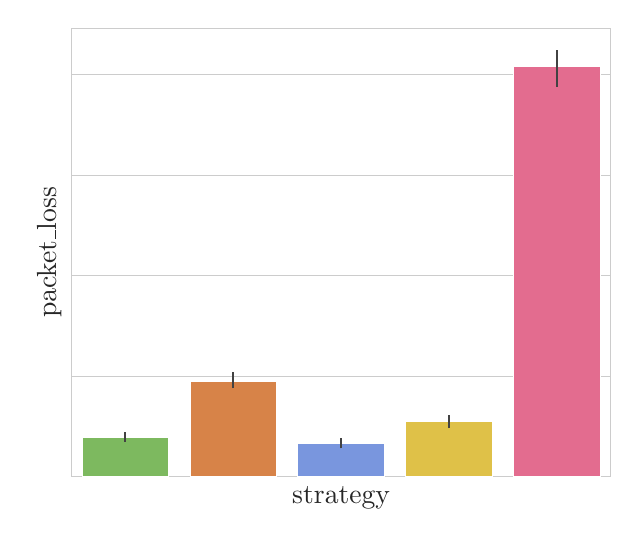
\begin{tikzpicture}

\definecolor{cornflowerblue121150222}{RGB}{121,150,222}
\definecolor{darkseagreen12518595}{RGB}{125,185,95}
\definecolor{darkslategray38}{RGB}{38,38,38}
\definecolor{darkslategray66}{RGB}{66,66,66}
\definecolor{lightgray204}{RGB}{204,204,204}
\definecolor{palevioletred227108143}{RGB}{227,108,143}
\definecolor{peru21513172}{RGB}{215,131,72}
\definecolor{sandybrown22319372}{RGB}{223,193,72}

\begin{axis}[
axis line style={lightgray204},
tick align=outside,
x grid style={lightgray204},
xlabel=\textcolor{darkslategray38}{strategy},
xmajorticks=false,
xmin=-0.5, xmax=4.5,
xtick style={color=darkslategray38},
xtick={0,1,2,3,4},
xticklabels={ofb,dynamic,static-1,every-10ms,every-100ms},
y grid style={lightgray204},
ylabel=\textcolor{darkslategray38}{packet\_loss},
ymajorgrids,
ymajorticks=false,
ymin=0, ymax=0.892779290460173,
ytick style={color=darkslategray38}
]
\draw[draw=white,fill=darkseagreen12518595,line width=0.32pt] (axis cs:-0.4,0) rectangle (axis cs:0.4,0.0788460877633071);
\draw[draw=white,fill=peru21513172,line width=0.32pt] (axis cs:0.6,0) rectangle (axis cs:1.4,0.189941246403281);
\draw[draw=white,fill=cornflowerblue121150222,line width=0.32pt] (axis cs:1.6,0) rectangle (axis cs:2.4,0.0656591706210027);
\draw[draw=white,fill=sandybrown22319372,line width=0.32pt] (axis cs:2.6,0) rectangle (axis cs:3.4,0.109801521377984);
\draw[draw=white,fill=palevioletred227108143,line width=0.32pt] (axis cs:3.6,0) rectangle (axis cs:4.4,0.817526094947463);
\addplot [line width=0.864pt, darkslategray66]
table {%
0 0.0695394430603759
0 0.0882443044053469
};
\addplot [line width=0.864pt, darkslategray66]
table {%
1 0.176026802322576
1 0.208031514326573
};
\addplot [line width=0.864pt, darkslategray66]
table {%
2 0.0562579054913693
2 0.0763076068530362
};
\addplot [line width=0.864pt, darkslategray66]
table {%
3 0.0965210185363295
3 0.12222934886771
};
\addplot [line width=0.864pt, darkslategray66]
table {%
4 0.775899240298922
4 0.85026599091445
};
\end{axis}

\end{tikzpicture}
